%!TEX root = ../NCVC6.tex

\mysection{CADでの作図とNCVCの読み込み}

\vspace*{1zh}
 図\ref{fig:sample.jww} のようなCADデータを準備します.
わかりやすくするために四角形の四隅にG54~G57のワーク座標原点を示す円を作図しました.
切削データはワーク座標原点との位置関係を基準に作図してください.

\begin{figure}[H]
\centering
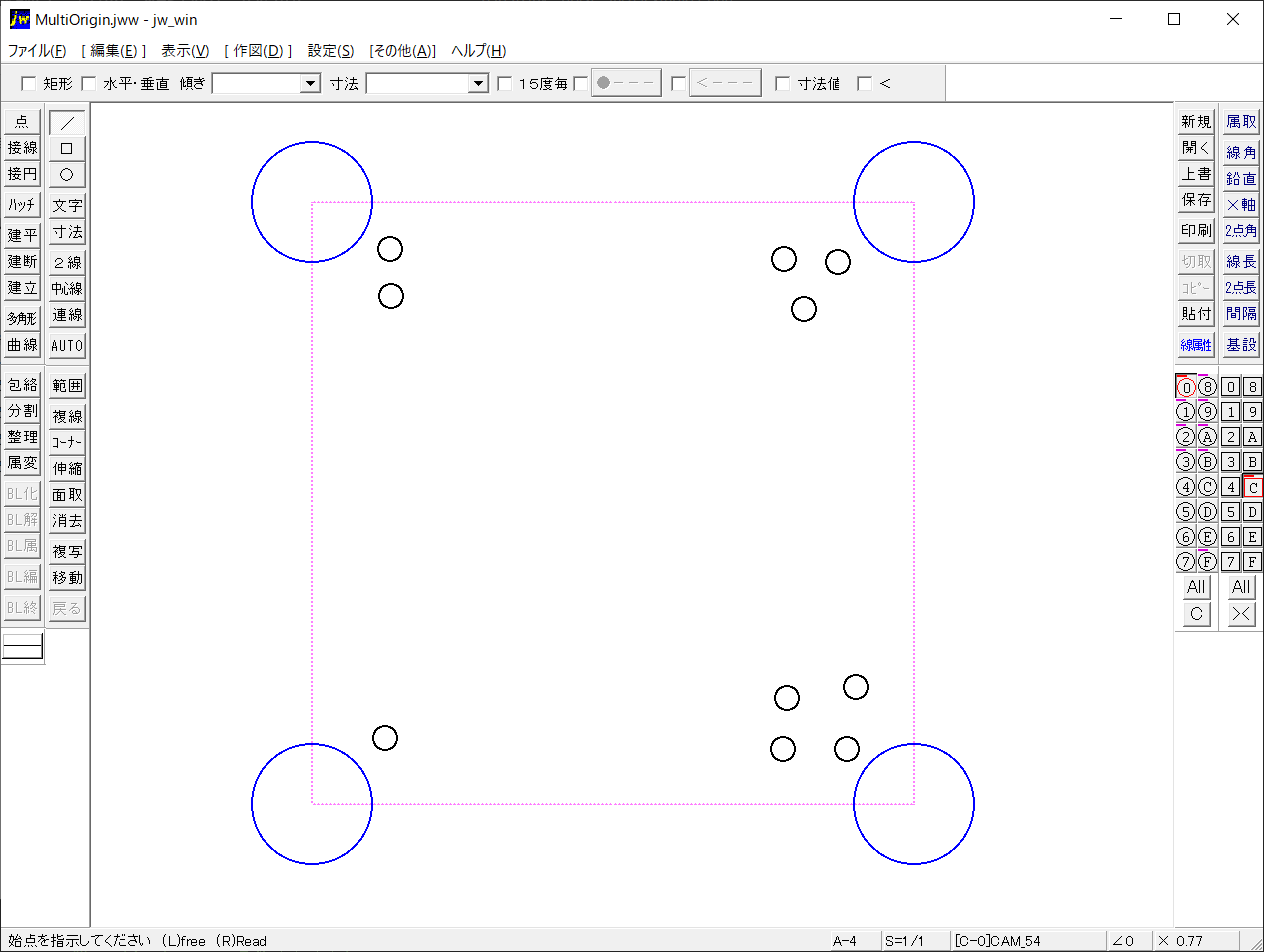
\includegraphics[scale=0.5]{No2/fig/sample.jww.png}
\caption{サンプル図形}
\label{fig:sample.jww}
\end{figure}

 レイヤ構成は図\ref{fig:layer} のようになります.
それぞれのワーク座標系の原点を示すレイヤに [ORIGIN\_xx] (xx:G54~G57) という名前を付けます.
切削レイヤも同様に [CAM\_xx] のように原点レイヤとの関連がわかるように名前を付けてください.

\begin{figure}[H]
\centering
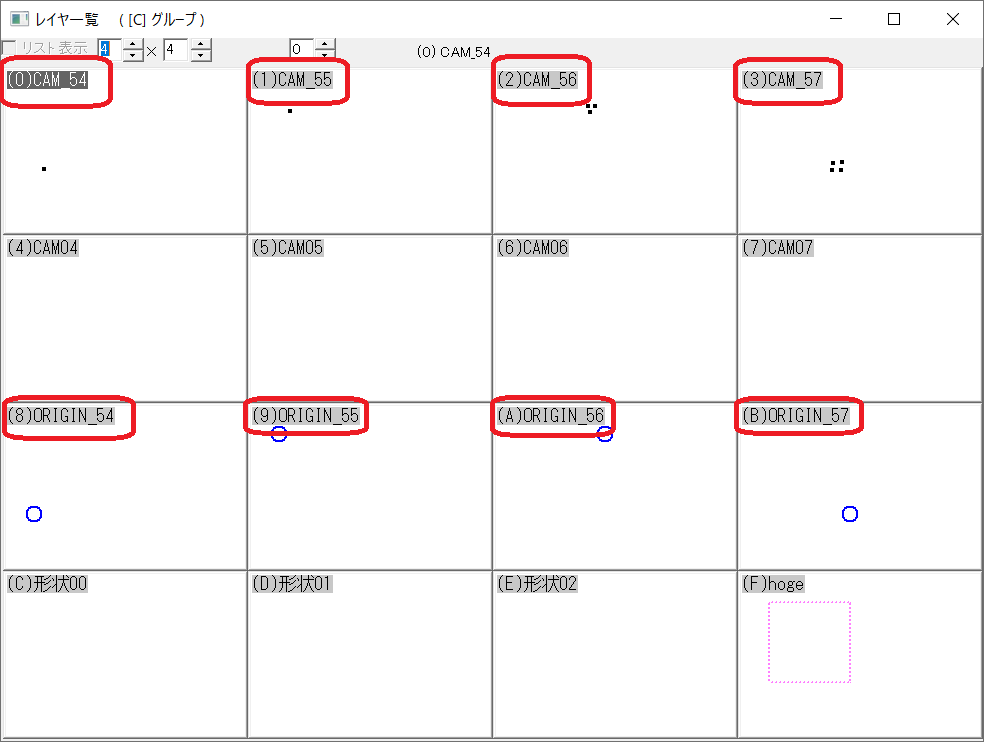
\includegraphics[scale=0.55]{No2/fig/layer.png}
\caption{レイヤ構成}
\label{fig:layer}
\end{figure}

 このデータをNCVCに読み込ませると図\ref{fig:read} のようになります.
[CADデータの読み込み設定]で[原点データがないとき]の設定が[エラー]になっているとエラーメッセージが表示されます.
エラー以外にしていると切削データの占有矩形から自動的に原点が設定されます.
図\ref{fig:read} の場合は[中央]の設定です.
この時点でのエラーや原点情報は無視してかまいません.

\begin{figure}[H]
\centering
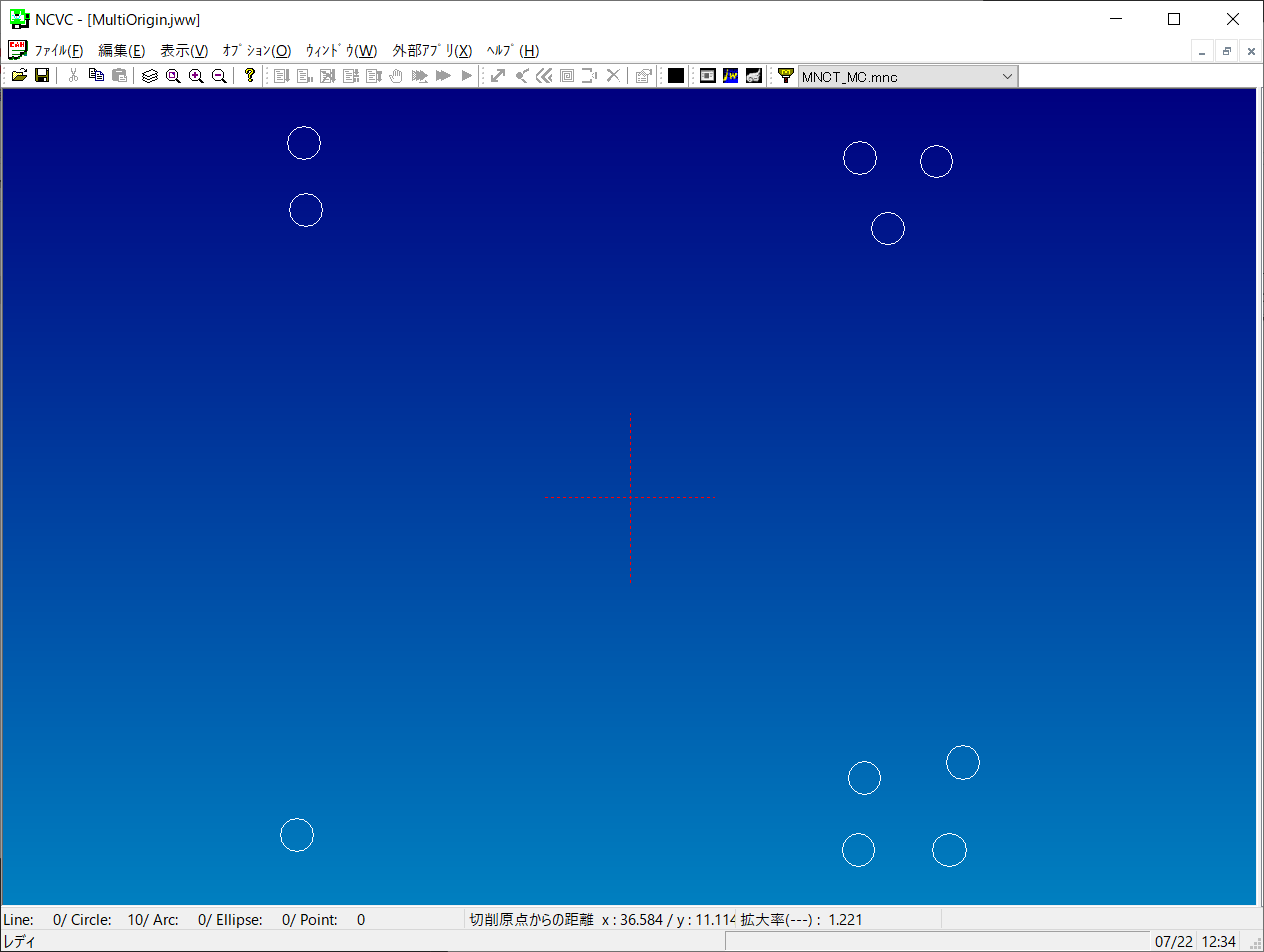
\includegraphics[scale=0.5]{No2/fig/read.png}
\caption{CADデータの読み込み}
\label{fig:read}
\end{figure}
